%!TEX root = ../dissertation.tex

\chapter{Solution}
\label{chapter:solution}


\section{Overview}
We set out to create an IDE for GD programming that is available from a web page.

There are four related tasks that the environment needs to support in order to be useful for the architect:
it needs to run programs; it needs to display their results; it needs to make it easy to see the traceability relationship between program and results; and it needs to export results to \gls{cad} applications.

To accomplish this, there are two separate components: (1) the web page, where the \gls{ui} for creating programs is; and (2) the remote CAD service, that offers an \gls{api} for running programs in \gls{cad} applications.
The first three tasks can be handled by the web page alone since there is no need to interact with the \gls{cad} applications running in the user's computer.
The forth task requires both the web page and the remote CAD service.

In the rest of the chapter we describe these two components and how each of the tasks is implemented.

We start by looking at the web page.


\section{Web page}
To handle the tasks of running programs, supporting traceability and displaying results, the web page has the layout shown in Figure~\ref{fig:page:view}.
Taking up most of the screen space are a text editor and a 3D view that allow the architect to edit a program and view results alongside it.
On top of these two are controls for running programs and for traceability data collection.
To the left is the interface for running programs in \gls{cad} applications and a list of the currently available programs.

%{\bf(describe high-level view of the inner workings of the page)}

\begin{figure}
  \centering
  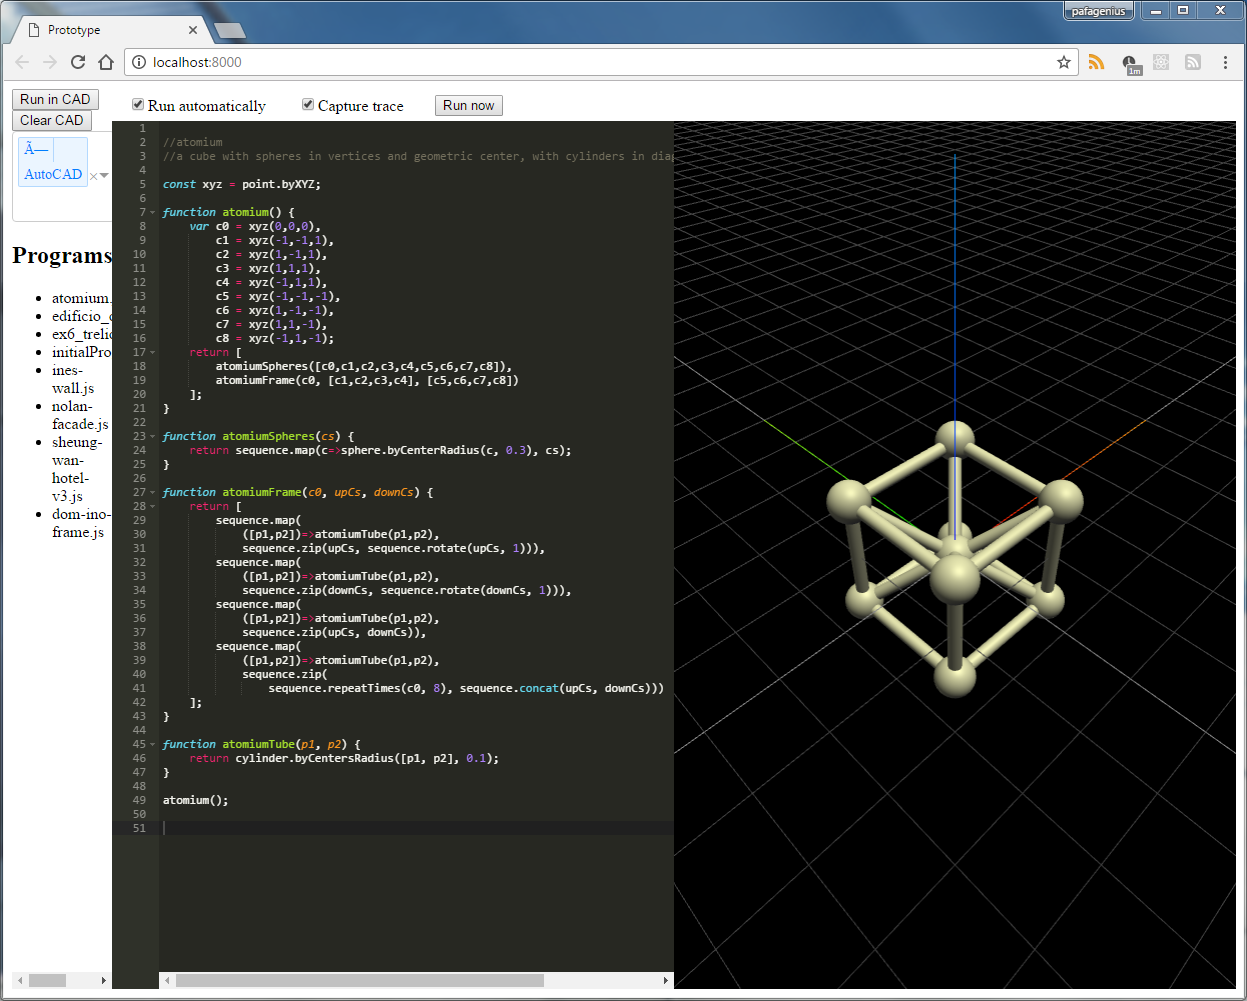
\includegraphics[width=12cm]{./images/webpage_view}
  \caption{An example view of the web page.}
  \label{fig:page:view}
\end{figure}


\subsection{Handling Traceability}
Traceability can be achieved by giving feedback to the programmer when he interacts with the program or the results.
The environment implements some mechanisms that allow it to give this feedback.

One of the ways the environment does this is by letting the programmer adjust literals more intuitively.
Afterwards, the environment reruns the program to show the effect of the adjustments.
It can also rerun the program whenever there is a change, like when a new statement is added to a function, an expression is changed, or when a new function is written.

The other way the environment provides traceability to the user is by showing it directly.
When the user points at a function call in the source code, the environment immediately highlights the shapes that it produced in the 3D view.


\subsubsection{Adjusting Literals}
\paragraph{Rationale for automating literal adjustment}
When a value, such as a number, is typed directly into a program's source code, it is called a literal value, or simply by literal.
When experimenting with a \gls{gd} program, architects find themselves repeatedly adjusting literals that were hardcoded into the program.
This is usually done by retyping parts of the literal's text with higher or lower digits.

Editing literals this way often leads to errors, since it is easy to mistype some characters.
One can increase their value by an order of magnitude if, by mistake, he inserts one character without removing another.
When increasing them in steps, different hand movements are required when there is carry over, yet again increasing both the likelihood of mistyping and the time it takes to make the changes.
These errors get amplified when the programming environment provides real time feedback and, like so, begins rerunning the program before the error is corrected, leading to reduced \gls{ui} responsiveness.

To make this interaction more user friendly and less prone to errors, we decided to simplify the task.
Instead of retyping the literal, the user can just ``Click and drag'' on the literal to change its value.

\paragraph{Implementation}
To implement this behavior, we need to focus on the program editor, as this is where the relevant information is.

The behavior starts when the user presses a mouse button while the pointer is over a numerical literal.
If it is indeed a numerical literal, we setup an event listener that will update the literal every time the pointer moves until the mouse button is released.

To check that the pointer is over a numerical node, we use the pointer position and the \gls{ast} of the current program with location data.
Since the program will change during the behavior, we keep the path taken through the \gls{ast} to the numerical literal.
We also keep the starting pointer position as a reference for calculating the new literal value when the mouse is moved.

We update the literal by changing the portion of the source code that it represents to the digits representing the new value.
The new value has the same number of fractional digits as the original literal.
To get the new value, we first extract the number of fractional digits and an integer containing the literal's digits and sign (ignoring the decimal point) from the literal's source text.
Afterwards, we add the horizontal distance between the starting point and the current pointer position to the number.
Finally, we convert it back to text and re-add the decimal point.

\paragraph{Alternative ways of adjusting literals}
There are several ways we can extend the user interface to make this more user friendly, and none of them rely on manually replacing digits.
They have a simpler mapping to the user's intent.
The following list describes some of them:

\begin{itemize}
  \item {\bf Virtual joystick} Clicking on a literal will display a virtual joystick close to it. When clicked and dragged, it changes the value repeatedly over time, being faster or slower depending on how much the handle is moved from its center.
  \item {\bf Click and drag} Clicking and dragging on a literal will change it according to how much the pointer moved from the starting position.
  \item {\bf Sliders} Clicking on a literal will display a slider. Dragging the slider's handle will change the literal depending on how much the handle is moved from the center of the slider. The slider can have different scales, linear or non-linear, to map the center-handle distance to the amount of change for the literal.
  \item {\bf Keyboard shortcuts} Pressing key combinations while having a literal selected, or the text editor's caret on it, will increment or decrement it.
\end{itemize}


\subsubsection{Program-Results Relationship}
Reducing the time between making a change and seeing its effect is one way to provide traceability.
However, traceability can also be actively shown by the environment.
If the programming environment takes care of tracking the relation between the program and results, the architect only needs to ask for the relation instead of having to track it by himself, freeing his mind to think about the problem.

There needs to be a way to give the architect quick access to the relation being tracked by the environment.
To do this, our solution highlights certain parts of the program and  its results when the pointer is on either one.
More specifically, when the pointer is over a part of the program, it highlights all the results that it produced;
when the pointer is over a part of the results, it highlights the part of the program where it was created.
Figure~\ref{fig:trace:example} shows an example for both of this cases.

\begin{figure}
  \centering
  
\includegraphics[width=12cm]{./images/traceability_example}
  \caption{Two examples of the traceability mechanism. The first from program to results and the second from results to program.}
  \label{fig:trace:example}
\end{figure}

Currently our solution only tracks the results produced by calls to functions.
This was a compromise to balance performance, since keeping track of traceability is an additional task that needs to be performed while running the program.

\paragraph{Alternative ways of showing traceability}
There are other ways for showing the relation between the program and its results.
We will describe some of them next.
\begin{itemize}
  \item {\bf Timetable} As described in Learnable Programming\cite{victor2012learnable}, making things visible makes them more real to the programmer. Timetables were proposed as a way to visualize the control flow of programs. They act as a map of the program's execution. By seeing the control flow, it is easier to see what the program does and it is easier to point at interesting locations. By allowing this, timetables provide better navigation inside a program's execution.
  \item {\bf Display data} Also described in Learnable Programming\cite{victor2012learnable}, displaying data would increase the amount of traceability the system provides. Apart from being able to see the control flow and the 3D results, seeing the other values (e.g. numbers, booleans) used throughout the program would give the programmer a more complete view of the execution.
\end{itemize}


\subsection{Running Programs}
One of the fundamental parts of the programming environment is that it runs programs.
To run programs, the environment needs to know which programming language is being used and which primitive operations the program has access to.
After knowing these, the environment must have a process to run the program and collect results so they can be displayed later.


\subsubsection{Program Structure}
Before a program can be run, the programming language has to be defined.
In our solution, we decided that it would be best to use JavaScript, as it was thought for designers and also because of its current performance in modern web browsers.
%{\bf(a source would help)}

However, there is a question: how do we get results from a program so we can display them?
Our solution uses the values of the top-level expression statements of the program as its results.

Listing~\ref{lst:program:example} gives an example of what a program looks like in our environment.

\begin{listing}
\begin{minted}[linenos,frame=lines]{js}
function abacus(height, side) {
  return box.byXYZ(side, side, height);
}

function echinus(height, side, neckSide) {
  return coneFrustum.byRadiusesHeight(neckSide, side, height);
}

function shaft(height, side, neckSide) {
  return coneFrustum.byRadiusesHeight(side, neckSide, height);
}

function column(height, side, neckSide) {
  return [
    translate(abacus(height*0.05, side)).byZ(height*0.95),
    translate(echinus(height*0.05, side, neckSide)).byZ(height*0.90),
    shaft(height*0.90, side, neckSide)
  ];
}

column(6.00, 0.8, 0.7);
\end{minted}
\caption{An example of a program written our environment.}
\label{lst:program:example}
\end{listing}


\paragraph{Alternatives for getting results}
There are other alternatives that could have been used.
For example:
\begin{itemize}
  \item {\bf Special entry point} Like in OpenJSCAD, we could require that every program must define a function with a special name (e.g. ``main''). The environment then calls this function and uses its results as the results of the program.
  \item {\bf Display function} Another way to get results from a program is giving access to an output function to the program. During its execution, the program calls this function, maybe several times, to produce its output.
  \item {\bf Imperative primitives} A third way to get results is by adding a side-effect to the 3D object producing functions/primitives. Apart from creating the object, they also add it to the program's results. This is similar to having a display function, as all primitives become specialized display functions.
\end{itemize}


%\subsubsection{Providing primitives / Runtime library / Primitive Library}
%\label{sub:provide:predefs}
%{\bf(what is the purpose of this subsubsection? I already talk about providing primitives in the next subsubsection...)}\\
%Any program needs to based upon functionality already provided by its host environment.
%It is this functionality that enables the program to produce results.
%
%But how does our solution do this for programs written by architects?
%We do this by defining all predefined functionality in a JavaScript module and then providing it to the function that represents the program as a parameter.
%Afterwards, we also add some code to the beginning of the program that will declare each primitive and extract the corresponding functionality from that parameter.


\subsubsection{Running process}
When the environment runs a program, it needs to do two things: (1) collect the results of the program; and (2) collect traceability data.
It does these two by instrumenting the program with additional calls to special functions that record the desired information.

To be able to perform the instrumentation, the environment parses the program using Esprima, a JavaScript parser\footnote{https://github.com/jquery/esprima (last accessed on 10/10/2016)}, to get its \gls{ast}.\footnote{The \gls{ast} conforms to a community standard. It can be found at https://github.com/estree/estree (last accessed on 10/10/2016).}

Afterwards, the \gls{ast} is transformed by: (1) adding a recording call to all top-level expression statements; and (2) adding a recording call to all function call expressions.
Figure~\ref{fig:instrument:example} exemplifies the transformation.

To let the recording functions know top-level expression or function call is producing a result, we also provide them identifiers for those expressions.

After this step, the environment creates a new function with the instrumented program as its body.
The primitives and recording functions are provided as parameters to this new function.

Finally, the newly created function is called and, afterwards, the recorded information is made available to the rest of the system.

\begin{figure}
  \centering
\begin{minipage}[t]{0.45\linewidth}
  \center{Before}
  \begin{minted}[frame=lines]{js}
let s = sphere.byRadius(5);
s;




  \end{minted}
\end{minipage}
\hspace{0.05\linewidth}
\begin{minipage}[t]{0.45\linewidth}
  \center{After}
  \begin{minted}[frame=lines]{js}
let s = recordCallResult(
   sphere.byRadius(5),
   /*function call ID*/);
recordTopLevelResult(
   s,
   /*top-level expression ID*/);
  \end{minted}
\end{minipage}
  %\includegraphics[width=1.0\textwidth]{./images/program_instrumentation}
  \caption{A program before and after the transformation.}
  \label{fig:instrument:example}
\end{figure}


%\subsection{Displaying Results}
%{\bf(interesting stuff about displaying results)}\\


\section{Remote CAD Service / Exporting to CAD}
The last task that the environment needs to support --- exporting to \gls{cad} --- requires it to communicate with \gls{cad} applications that are installed in the architect's computer.
Unfortunately, web pages are not allowed to communicate with applications running in the computer displaying them.

To overcome this restriction, we have implemented an application that the architect must install and run in his computer.
This application serves as a bridge between \gls{cad} applications installed in the computer and the environment running in the web page.
After being started, the application detects which \glspl{cad} are installed in the computer and connects to the ``environment directory'' so it can be discovered by the web page.
When the architect needs to export a program to his \gls{cad}, the web page connects to the application in his computer through the ``environment directory'' and starts to send requests to it, in order to create shapes in the \gls{cad}.

Figure~\ref{fig:remote:cad:example} shows an example of this functionality.
The architect has created a program using the web page environment.
After selecting AutoCAD and SketchUp as export destinations, he starts the export process and, some time later, the model resulting from running the program is available in both \gls{cad} applications.

Please note that it is only needed to install the application when the architect is finally ready to get the program's results on a \gls{cad}.
Furthermore, the application only needs to be installed in the computer that actually has the \gls{cad} installed, while the rest only accesses the web page.


\subsection{Implementation}
We implemented the application as a small Racket server.
It expects to receive HTTP requests for adding shapes to the currently selected \glspl{cad}.
It also expects requests for specifying what \glspl{cad} should the shapes be added to and for deleting all shapes they may have.
%{\bf(appendix has remote CAD service API?)}

Apart from the connection application and web page, there also needs to be a connection between the application and the \gls{cad} applications.
Different \glspl{cad} have different \glspl{api} so the application needs to know how to interact with each one.

Instead of implementing the connection with \gls{cad} applications installed in the computer, the application uses Rosetta as an intermediate.
This way, it only has to correct the semantic differences between Rosetta's \gls{api} and the remote CAD service's \gls{api}.

We chose to temporarily host the web page containing the \gls{ide} in the application.
Using this setup, it is easier to test the communication between the page and the application.
This setup also avoids dealing with cross-origin restrictions imposed by web browsers for \gls{ajax} requests.

\begin{figure}
  \centering
  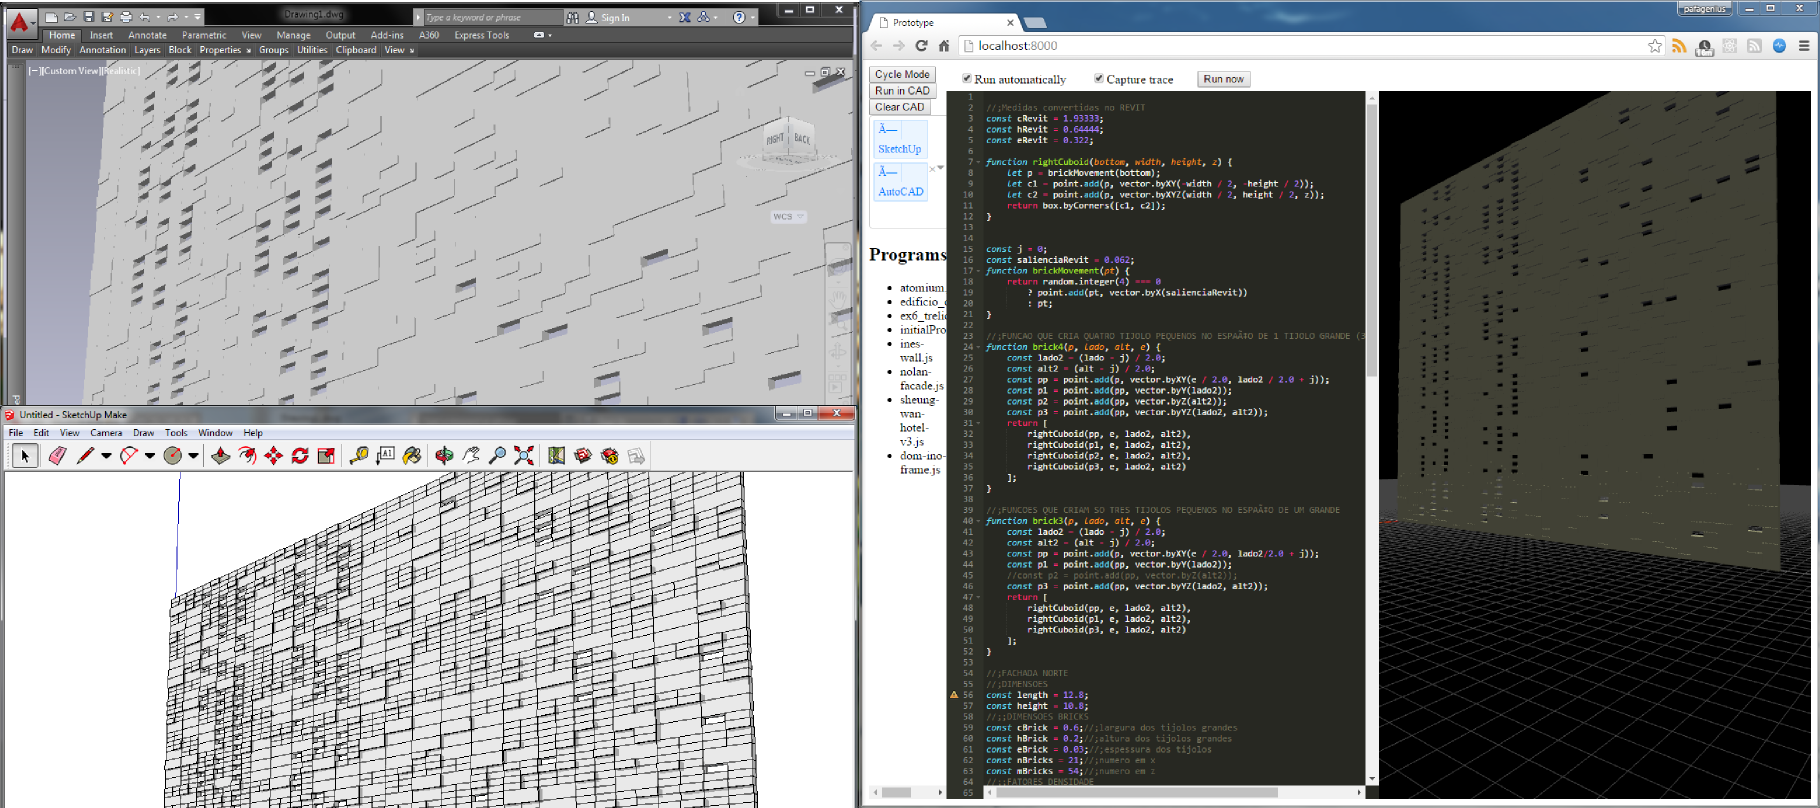
\includegraphics[width=1.0\textwidth]{./images/remote_cad_example}
  \caption[An example of the remote CAD service.]{An example of the remote CAD service. The results of the program have been passed to both AutoCAD and SketchUp.}
  \label{fig:remote:cad:example}
\end{figure}


%Design principles / Guiding ideas
%- Ideas based on observations from related work?

%Architecture - Show the overview of the architecture
%- Web page + remote CAD service

%Web page
%- Architecture
%- Page Layout
%- Features / What needs to be done by the IDE?
%   - Discussion + Decision
%   - Implementation
%- Problems
%   - Adjusting source code values
%   - Instrumenting and running programs
%     - Getting results / What is a program?
%     - Providing primitives/predefined bindings
%     - Handling traceability
%   - (Running programs blocks the UI)
%   - Displaying 3D results

%Remote CAD service
%- Architecture
%- Problems
%   - Supporting multiple CADs
%   - Defining the API

%Problem: Handling CAD communication
